\chapter{Introduction}

\begin{changemargin}{1.0cm}{1.0cm} 
\abstractpreamble{Several \acrshort{gen3+} nuclear reactors have been proposed for construction in the UK and \acrshort{gen4} nuclear reactors are being researched and developed.  At the time of writing Hinkley Point C is under construction and Sizewell C has had government approval.  However, much more must be done to ensure the energy security of our nation.  Well established reactor types and exciting new designs could contribute to solving this problem, but challenges to materials science must be overcome.\\
\\
New materials are required to withstand the extreme conditions in and around the core of these reactors.  Austenitic stainless steels have been an important structural material in the industry, and may continue to be so, providing the problem of \acrfull{igscc} can be addressed.  Doping these steels with \acrfull{pgm}s has been seen to reduce \acrshort{igscc}, but the effects on corrosion resistance are unknown for these steels when irradiated by a radiation field.}
\end{changemargin}



%%%%%%%%%%%%%%%%%%%%%%%%%%%%%%%%%%%%%%%%%%%%%%%%%%%%%%%%%%%%%%%%%%%%%%%%%%%%%%%%%%%%%%%%%%%%%%%%%%%%%%%%%%
%%
%%  MOTIVATION
%%
%%%%%%%%%%%%%%%%%%%%%%%%%%%%%%%%%%%%%%%%%%%%%%%%%%%%%%%%%%%%%%%%%%%%%%%%%%%%%%%%%%%%%%%%%%%%%%%%%%%%%%%%%%

\section{Motivation}

Mass produced steels are not perfect repeating crystals, but are made up of small grains.  \Gls{Cr} is added to steel to make stainless steel, and this is more resistant to corroding than steel.  When steel is in a nuclear reactor, it will have to perform under extreme conditions, such as:

\begin{itemize}
\item high temperatures
\item strain cause by high pressures and radiation induced swelling
\item radiation damage and strains resulting from this damage
\item a changing environment (radiolysis, isotope transmutation)
\item corrosive environments while in the reactor
\item corrosive environments out of the reactor (e.g. fuel cladding in storage)
\end{itemize}

Radiation damages the steel in a number of ways including directly knocking atoms out of place within the lattice, changing the environment (e.g. radiolysis) and transmuting isotopes.  An example of the latter is a neutron transmuting an \Gls{Fe} atom into a \Gls{Co} atom.

In time, the radiation damage causes the percentage of Cr at the grain boundaries to drop, and as it falls the steel loses its protection from corrosion at the boundary between the grains it is made of.  

This work is divided into two parts.

\subsection{Part 1: Activity Computer Program}

The materials must be tested before being used in a nuclear reactor.  One way to do this would be to place samples of the steel into a test reactor.  This is expensive and, as a by-product, the steel sample becomes radioactive.  It is difficult to create a large number of neutrons, but it is much easier, and cheaper, to create a beam of protons.  Protons can be accelerated in a machine such as the Cyclotron at the University of Birmingham.  

The damage that protons cause to a sample is not precisely the same as that cause by neutrons, but it is a cheaper alternative and is a trade-off between the cost and results.  One side effect that proton irradiation shares with neutron irradiation is the creation of radioactive waste.  

The first part of this work investigates exactly how radioactive a samples becomes when irradiated with a proton beam.  An existing equation, named after Mathematician Harry Bateman\cite{bateman}, was modified and a computer program was created to perform the calculation.  The user inputs the constituent elements that make up the material, the ratio of these elements, and the irradiation settings.  The program then estimates how radioactive the sample will be and the predicted gamma energies.


\subsection{Part 2: Iron-Palladium and Iron-Ruthenium Potential}

The addition of \Gls{Cr} to make stainless steel is not the only way to make a steel resistant to corrosion.  Adding metals such as \Gls{Mo}, \Gls{Pd} and \Gls{Ru} to steel can increase the resistance to corrosion, but Mo is several hundred times the cost of Fe ore, and Pd is thousands of times as expensive.

Simulating radiation damage using a computer is now a feasible and sensible way to investigate how these materials will be affected by radiation damage, and the simulations may reveal insights that experiments are not able to show, either because they happen on too small a timescale or within the material at too small a length scale.

Key to the simulations success is being able to accurately calculate how the atoms interact with one another.  The second part of this work concentrates on deriving a mathematical description of how Pd \& Fe and Ru \& Fe atoms interact with one another, which would then allow future simulations of steel with small amounts of Pd or Ru added to it.

Radiation causes Cr to be depleted at the grain boundary.  If these simulations go on to show that Pd and Ru are not depleted, it would suggest that the corrosion resistance is maintained despite the decrease in the amount of Cr at the grain boundary due to radiation damage.


%%%%%%%%%%%%%%%%%%%%%%%%%%%%%%%%%%%%%%%%%%%%%%%%%%%%%%%%%%%%%%%%%%%%%%%%%%%%%%%%%%%%%%%%%%%%%%%%%%%%%%%%%%
%%
%%  BRIEF HISTORY, PRESENT AND FUTURE
%%
%%%%%%%%%%%%%%%%%%%%%%%%%%%%%%%%%%%%%%%%%%%%%%%%%%%%%%%%%%%%%%%%%%%%%%%%%%%%%%%%%%%%%%%%%%%%%%%%%%%%%%%%%%


\FloatBarrier
\begin{comment}
\section{Nuclear Power in the United Kingdom}

\subsection{Nuclear Fuel}

The primary fuel of commercial nuclear power stations since those first built in the 1950s has been \Gls{U}.  ${}^{235}_{92}U$ is \gls{fissile} and fissions with a high probability when thermal neutrons are captured, due to its very high thermal neutron fission cross section (fig. \ref{figure:u235u238fissionxs}).

\begin{figure}[tbp]
  \begin{center}
    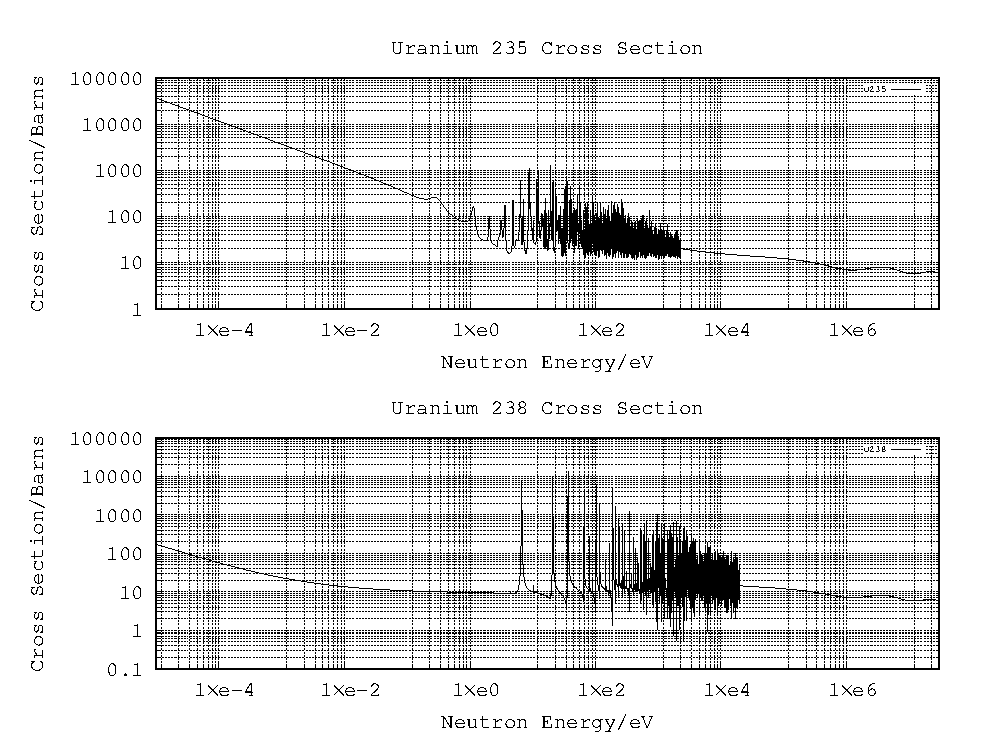
\includegraphics[width=.8\linewidth]{chapters/introduction/plots/uranium_cross_section/u_xs}%
    \caption{U-235 and U-238 fission cross sections plotted from the JEFF 3.3 data file\cite{jeff33}}
    \label{figure:u235u238fissionxs}
  \end{center}
\end{figure}

Natural U contains a small percentage of fissile ${}^{235}_{92}U$ (0.7\%) with the rest being its heavier isotope, ${}^{238}_{92}U$.  This heavier isotope is \gls{fissionable}, but its thermal fission cross section is much lower than ${}^{235}_{92}U$ (fig. \ref{figure:u235u238fissionxs}).  Many of the design considerations for reactors in operation revolve around the amount of ${}^{235}_{92}U$ there is in the fuel and having a sufficient flux of thermal neutrons passing through the fuel to sustain a reaction.

A number of \acrshort{gen4} designs use the fast neutron spectrum to fission ${}^{238}_{92}U$ and other fuels such as ${}^{232}_{90}Th$ to generate energy and breed other fissile isotopes (${}^{233}_{92}U$).  By moving away from ${}^{235}_{92}U$, this increases the potential fuel stockpile, but also brings its own set of challenges.


\FloatBarrier

\subsection{Generation I Reactors}

The first generation reactors were primarily prototype reactors.  They included graphite moderated reactors, light water and heavy water reactors.  Early reactors were designed to produce electricity, but also fissile material for nuclear weapons.  With a power output of less than 2MW, the Gen I power station Calder Hall generated much less electricity than a modern nuclear power plant which may produce 1GW per reactor.  It did, however, produce \Gls{Pu} for the UK's nuclear weapon programme.

Magnox type reactors were the first used in the \acrshort{uk}.  These reactors used natural U as a fuel and were carefully designed to produce energy despite using an un-enriched fuel.  Graphite was used as a moderator, and the low neutron capture cross section of the Magnox \Gls{Mn} alloy cladding allowed a nuclear reaction to occur despite the fuel not being enriched.

In all there were 11 Magnox power stations built in the UK with 26 reactors in total.  Construction of the first commercial reactor in the UK, Calder Hall, started in 1953 and it operated from 1956 to 2003.  All have now shut down with the last, Wylfa in Anglesey, closing in 2015.

\subsection{Generation II Reactors}

\acrshort{gen2} marked the transition from prototype reactors to higher powered commercial reactors.  There were a number of designs including the \acrshort{agr}, a graphite core $CO_2$ cooled reactor, that was implemented in the UK.  Light water reactors included the \acrshort{pwr} and \acrshort{bwr} in the west and the \acrshort{vver} in the \acrshort{ussr}.  The \acrshort{rbmk} was a graphite moderated reactor used in the \acrshort{ussr} and the \acrshort{candu} a heavy water reactor designed and used in Canada.

There are many of these reactors from this period still in operation around the world, and there have been recent implementations of these designs.  When I started writing this thesis there were 15 reactors operational in the UK.  As of 2022 there are only 9 reactors currently operating in the UK, and they are all \acrshort{gen2} reactors.  Of these, 8 are \acrshort{agr} and 1, Sizewell B, is a \acrshort{pwr} (fig. \ref{fig:remainingreactorsuk}).  Perhaps this says something about the amount of time I have taken to complete this work, but it also highlights the loss of 40\% of the reactors we had within a decade, and this is concerning.

\begin{figure}[tbp]
  \begin{center}
    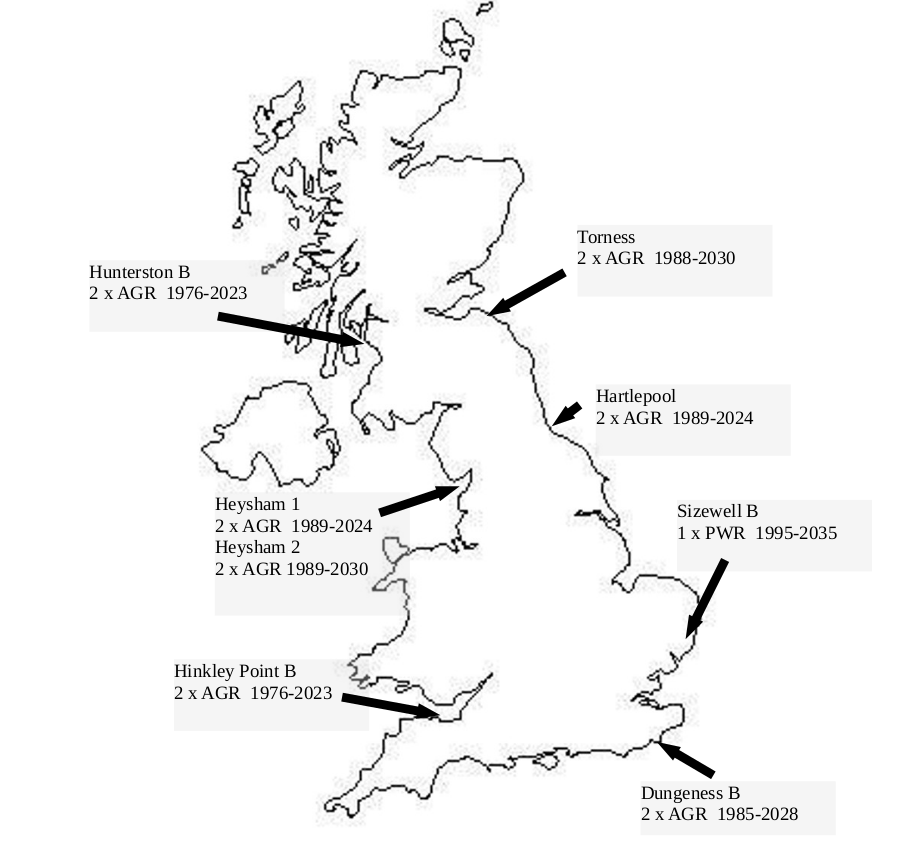
\includegraphics[width=12.0cm]{chapters/introduction/images/remaining_plants.png}
    \captionsetup{font={it}}
    \caption{Remaining reactor locations in the UK.  Active as of 2022: Heysham (4 x \acrshort{agr}), Torness (2 x \acrshort{agr}), Hartlepool (2 x \acrshort{agr}), Sizewell B (1 x \acrshort{pwr}) \cite{nuclearpoweruk}}
    \label{fig:remainingreactorsuk}
  \end{center}
\end{figure}

The planned life span for this generation of reactor was 30-40 years, although this has now been extended to 50-60 years in some cases.  The \acrshort{agr} reactors in the UK have been operational for over 40 years, with Hunterston B and Hinkley Point B being operational for 46 years before their service came to a close.  Designed with safety improvements in mind over Gen I reactors, they were also intended to produce more power with less of a focus on producing fissile material for weapons.  Unfortunately, this generation of reactors had the worst track record of any regarding safety, with Three Mile Island, Fukashima and Chernobyl all being \acrshort{gen2} designs.

\acrshort{gen2+} reactors have been built recently with 18 CPR-1000s being constructed over the last decade in China.  The UK is currently looking towards \acrshort{gen3+} reactors while \acrshort{gen4} proposals are being researched.   


\subsection{Generation III Reactors}

There are no \acrshort{gen3} reactors operating in the UK.  The first was built in Japan in 1996 and the type of reactor installed was an \acrfull{abwr}.  Bradwell B is a proposed site for the \acrshort{gen3} Hualong One type \acrshort{pwr} power plant (\acrshort{hpr}1000), and if this goes ahead it would have an expected opening date between 2030-2035.   

This generation of reactor was designed to exceed the service life of the previous generation, and generate power for at least 60 years.  The safety features have been improved and include increased resilience to external factors, including accidental or intentional aircraft collision into the plant\cite{genIIIimprovements}.

\acrshort{gen3+} reactors go further in adding passive safety features, such as natural circulation and gravity coolant feed \cite{geniiiplussafety}.  Other aims of future generations are to standardise and simplify designs whilst improve the economy over \acrshort{gen2+} and \acrshort{gen3}. 
\end{comment}

\section{An Approaching Energy Gap for the UK}

Since Calder Hall, the first commercial nuclear power plant, opened in 1956, the demand on electrical power generation in the UK has tripled (fig \ref{fig:electricityusagesuk}).  There is now a reliance on cheap and clean power from nuclear reactors as these have provided a quarter of our electricity until recently.

\begin{figure}[!h]
  \begin{center}
    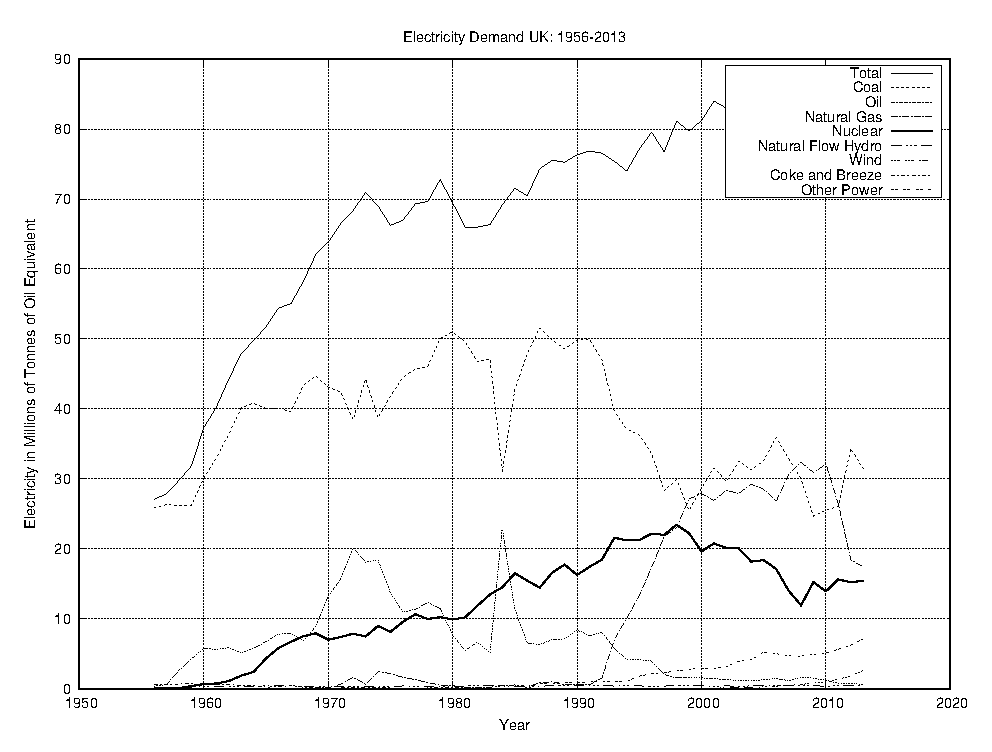
\includegraphics[width=.7\linewidth]{chapters/introduction/plots/elec_demand/elec_demand.eps}
    \captionsetup{font={it}}
    \caption{Electricity in Millions of Tonnes of Oil Equivalent\cite{ukpowerdata}}
    \label{fig:electricityusagesuk}
  \end{center}
\end{figure}

There is an obvious concern that within the next ten years the UK will lose a sizeable proportion of its electricity generation capabilities.  There are increasing pressures on countries to reduce their carbon dioxide output, so the gap created by ageing nuclear plants and coal power needs to be filled.


\subsection{Why choose Nuclear Power?}

As a civilization we need energy, whether it's in the form of electricity or stored chemically, and whilst we are becoming more efficient at using that energy, the demand for it will remain (unless something drastically changes our society).  There is a choice between burning fossil fuels or bio fuels, using energy from the Sun, wind, ground, oceans or rivers and finally using the energy of the nucleus, whether by fission or fusion.

Each has its drawbacks and advantages.  Renewable energies are unreliable; wind power only provides energy when there is a wind, and if the wind is too strong, they must be shut down or risk damage.  The Sun is only available for a portion of the day, and the duration and intensity change with the seasons, not to mention the impact of clouds on solar power.  Renewable sources are not very good at responding to demand; there isn't a button to turn up the power of the Sun, or increase the velocity of the wind when the national grid demands it.  If we were completely reliant on renewable energies, there would either need to be an efficient way to store energy on a large scale, or many more solar, wind, tidal and hydroelectric power stations than would be needed to produce excess energy.  Whilst the energy source may be free, turbines, solar panels, dams and so on require maintenance, so an excess of these would be wasteful and costly.

Fossil fuels release carbon dioxide, sulphur dioxide, naturally occurring trace radioactive elements and other pollutants into the atmosphere.  These power plants are useful because the fuel is cheap, but the waste is put back into the environment without much processing and the energy produce may be varied to meet the demand of the national grid.  

Nuclear power has a bad reputation with the public, in part caused by accidents such as the Windscale fire, Three Mile Island, Chernobyl, and Fukushima.  There have been examples of poor handling of nuclear waste in the past, such as the legacy storage ponds at Sellafield, and long term storage in geologically stable areas is something that hasn't been achieved to store the existing waste, let alone waste created in the future.

Modern nuclear power plants are very expensive to build, with the proposed 3.2GWe Sizewell C power plant expected to cost £20 billion or more \cite{ftnppcost}.  When compared to \textsterling0.5 billion for the 0.884GWe Carrington \acrshort{ccgt} Power Station \cite{efgccgtcost}, the initial costs are \textsterling0.57 billion per GWe for \acrshort{ccgt} compared to \textsterling6.25 billion per GWe for Nuclear.

There is an effort around the world of countries aiming to reduce the production of carbon dioxide as a result of burning fossil fuels.  When a power plant is operational, the carbon dioxide produced by nuclear power is negligible when compared with gas, oil and coal power plants.  

\begin{figure}[!h]
  \begin{center}
    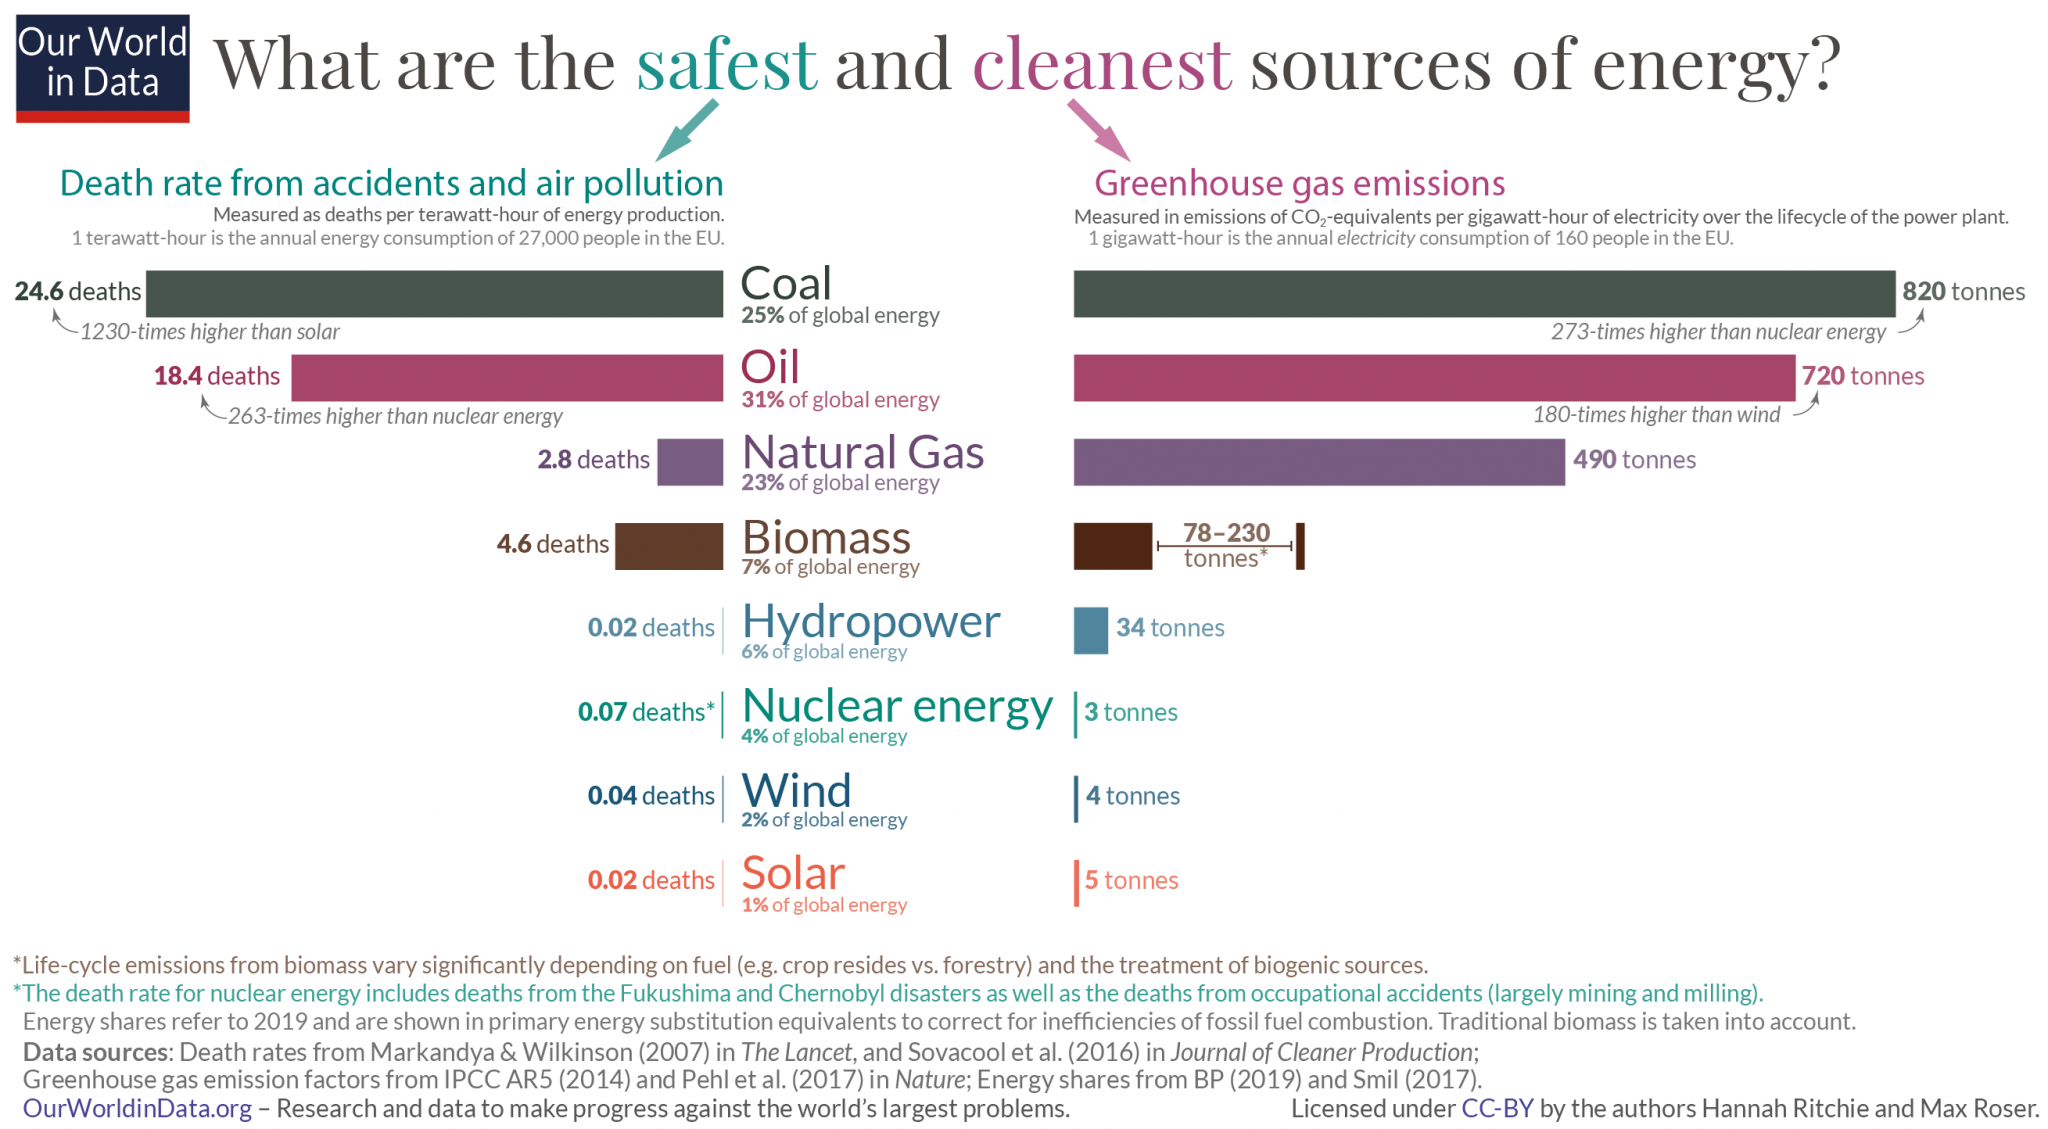
\includegraphics[width=.95\linewidth]{chapters/introduction/images/safest.png}
    \captionsetup{font={it}}
    \caption{Safest and cleanest sources of energy \cite{deathsfromenergysource} - deaths per terawatt hour and tonnes of CO\textsubscript{2} per gigawatt hour}
    \label{fig:safestenergy}
  \end{center}
\end{figure}

Despite its reputation amongst the public, nuclear is much safer than fossil fuels and is on par with renewable energies.  The pollution caused by fossil fuels affects us all and is responsible for many deaths each year, causing more misery than nuclear power ever has (fig. \ref{fig:safestenergy}).  Coal and oil are responsible for 350 and 260 times as many deaths as nuclear, respectively.

As a species, we have used combustion of chemicals to generate heat for thousands of years, culminating in high efficiency \acrshort{ccgt} power stations, with efficiencies above 60\%.  We are at the beginning of our journey with nuclear power, with many new and innovative designs proposed, where safety to plant workers and the general public are a priority.

Future designs may help to tackle the problematic waste generated in the past, and by using fertile material to produce fissionable elements other than ${}^{235}_{92}U$, the amount of fuel available to reactors will increase. 


\subsection{Proposed Generation III+ Nuclear Power Plant Designs}


\subsubsection{Areva \acrshort{epr}}

The 1.6GW Areva \acrshort{epr} design has four primary loops transferring heat by pressurised water from the reactor to heat exchangers.  It requires U enriched to 5\% ${}^{235}_{92}U$ in the form of U Oxide Pellets.  The inlet temperature is $568.75K$ and the outlet temperature is $602.95K$.

There are 241 fuels assemblies, each containing 265 fuel rods giving a total of 63865 rods.  The fuel rod cladding is made from 316 stainless steel and has an inner diameter of 7.72mm and an outer diameter of 9.68mm.  The materials used to construct the control rod drive mechanisms includes 410 stainless steel and 304 stainless steel.

There are two \acrshort{epr} reactors planned for the proposed Sizewell C power plant and they will be designed to produce a combined power output of 3.2 GWe.  The government has authorised planning consent for the power station and hopefully construction will start within the next couple of years.


\subsubsection{Westinghouse AP1000}

The 1.1GW Westinghouse AP1000 design is a pressurised water reactor with two primary loops transferring heat from the reactors to heat exchangers.  An enriched $UO_2$ fuel, up to 5\% ${}^{235}_{92}U$, is clad in Zirlo (a proprietary \Gls{Zr} alloy).  Zirlo is an alternative cladding material to 316 stainless steel, and as a cladding material is absorbs fewer neutrons that steel cladding.  The inlet temperature is $552.55K$ and the outlet temperature is $597.85K$ which is close to the temperature range of the \acrshort{epr}.  The composition of the control rod absorber material includes 304 stainless steel.

\begin{table}[h]
\begin{center}
\renewcommand{\arraystretch}{1.2}
\begin{tabular}{c c c}
\hline\hline
Property & 316SS Fe 20Cr 8Ni 1Mo & Zirlo (Hill Approximaton) \\
\hline\hline
Bulk Modulus (GPa)     & 164.9 \cite{elasticprofecr}  & 98.5 \cite{crystengcommzirlo} \\
Shear Modulus (GPa)    & 74.6 \cite{elasticprofecr}   & 33.2 \cite{crystengcommzirlo} \\
Young's Modulus (GPa)  & 194.3 \cite{elasticprofecr}  & 89.7 \cite{crystengcommzirlo} \\
Poisson's Ratio        & 0.30 \cite{elasticprofecr}   & 0.35 \cite{crystengcommzirlo} \\
\hline\hline
\end{tabular}
\end{center}
\caption{Bulk, shear, Young's modulus comparison: Zirlo and austenitic stainless steel }
\end{table}











\subsection{Generation IV}

\subsubsection{Goals of Generation IV Reactors}

The GenIV International Forum has put forward four main goals for this next generation of nuclear power\cite{genivgif}:

\begin{itemize}
\item sustainability
\item safety and reliability
\item economics
\item proliferation resistance and physical protection
\end{itemize}

The selection of known materials, and the development of new materials, will play a key part in all four of these goals.


\subsubsection{Carnot's Theorem}
\label{section:carnottheorem}

Whatever the motivation, whether it is to increase profits or to supply energy at greater amounts and for less cost to the consumer, increasing the efficiency of energy production is critical.  Solar panels are continually being improved to edge closer to their theoretical limit and wind turbines are being constructed larger and with more advanced materials to extract as much energy from the wind as possible.

In the same way, power plants that use heat are constantly being developed to improve efficiency.  In the nineteenth century Carnot showed that the maximum possible efficiency of a heat engine is determined by the difference in temperature between the heat reservoirs.\cite{carnottheorem}

\begin{equation}
\begin{split}
\eta_{max} = 1 - \frac{T_c}{T_h}
\end{split}
\end{equation}

To increase maximum efficiency, the temperature difference should be increased, and this leads to higher temperature reactors.  There will be a trade off between the increased temperature, the ability of the materials to withstand the temperature, health and safety considerations, the lifetime of components, the effect on the coolant and more.

The first generation of reactors in the UK were the gas cooled Magnox reactors.  With core temperatures of approximately $620K$\cite{magnoxtemp}, the thermodynamic efficiency  was relatively poor.  This was limited by the $MgO$ cladding, which was in turn selected due to the fuel.  Combined cycle gas turbines have much higher temperatures within their turbines, and the temperature of the steam within the secondary steam turbine can reach $850K$\cite{ccppwiki}, significantly higher than in a Magnox reactor.

The second generation of power plants, particularly in the UK, included the advanced gas reactor that used $CO_2$ as a coolant.  This reactor design increased temperatures to over $870K$, and thus the maximum possible thermodynamic efficiency was increased.

Several \acrshort{gen4} reactors have designed operating temperatures that exceed those of the \acrshort{agr}, and this brings a new set of challenges to overcome.



\subsubsection{Fast Reactors}

Examples of thermal neutron reactors include Magnox, \acrshort{agr}, LWR and Candu reactors.  These reactors contain moderators, designed to slow neutrons, decreasing their energy to thermal temperatures and leveraging the large neutron fission cross section of ${}^{235}_{92}U$.  The cross section for fast neutrons and ${}^{235}_{92}U$ is in the region of 1 barn, but thermal neutrons and ${}^{235}_{92}U$ have a fission cross section of over 1,000 barns.

\begin{figure}[!h]
  \begin{center}
    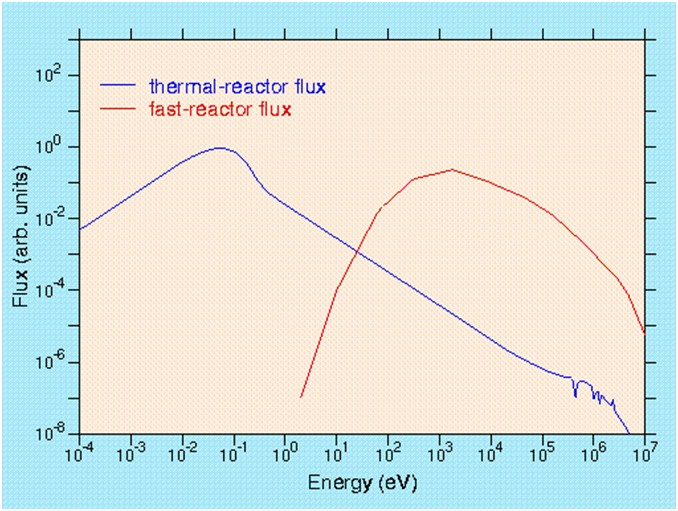
\includegraphics[width=7.0cm]{chapters/introduction/images/reactor-flux.png}
    \caption{Typical reactor flux - thermal and fast spectra \cite{thermalfastflux}}
    \label{fig:flux1}
  \end{center}
\end{figure}

Natural U contains 0.7\% ${}^{235}_{92}U$ and 99.3\% ${}^{238}_{92}U$\cite{uraniumenrichment}.  The thermal fission cross section for ${}^{238}_{92}U$ is small for thermal neutrons, and can be measured in the microbarn to millibarn range, but it has a much higher fission cross section with fast neutrons with a cross section closer to 1 barn for neutrons with an energy of 1MeV or more.  The neutron flux in a fast reactor is spread over a higher energy band than that of a thermal neutron reactor (fig. \ref{fig:flux1}).

Fast neutron reactors have been tested and used since the 1950s, and there are several \acrshort{gen4} reactor designs based on this approach.  Given the much larger percentage of ${}^{238}_{92}U$ in natural U, Fast Neutron Reactors have a larger stockpile of fuel.  They also breed fissile isotopes, ${}^{239}_{94}Pu$ and ${}^{241}_{94}Pu$.  This has its advantages and disadvantages.  The advantage is clear, as it produces fissile fuel as it runs, but the creation of fissile materials is a concern as these isotopes could be used in nuclear weapons.

\subsubsection[Lead-cooled Fast Reactors]{\acrlong{lfr}}

Light elements such as the hydrogen in water molecules, or carbon in a graphite stack, allow neutrons to efficiently lose energy.  When neutrons scatter inelastically with heavier elements, such as lead, they lose a much smaller percentage of their energy (fig. \ref{fig:inelasticscattering}).

The \acrfull{lfr} uses lead as the coolant.  Lead has a low reaction cross section and, because of its mass relative to a neutron, the kinetic energy lost in collisions is low, keeping more neutrons in the fast energy group.  As the coolant is a liquid, and the boiling point of lead is over $1,970K$, the system will run at atmospheric pressures and any problems associated with void formation due to boiling are removed.  The molten lead will act as a gamma shield and it will be chemically less reactive than the coolant in a \acrfull{sfr} or \acrfull{scwr}.

\begin{figure}[!h]
  \begin{center}
    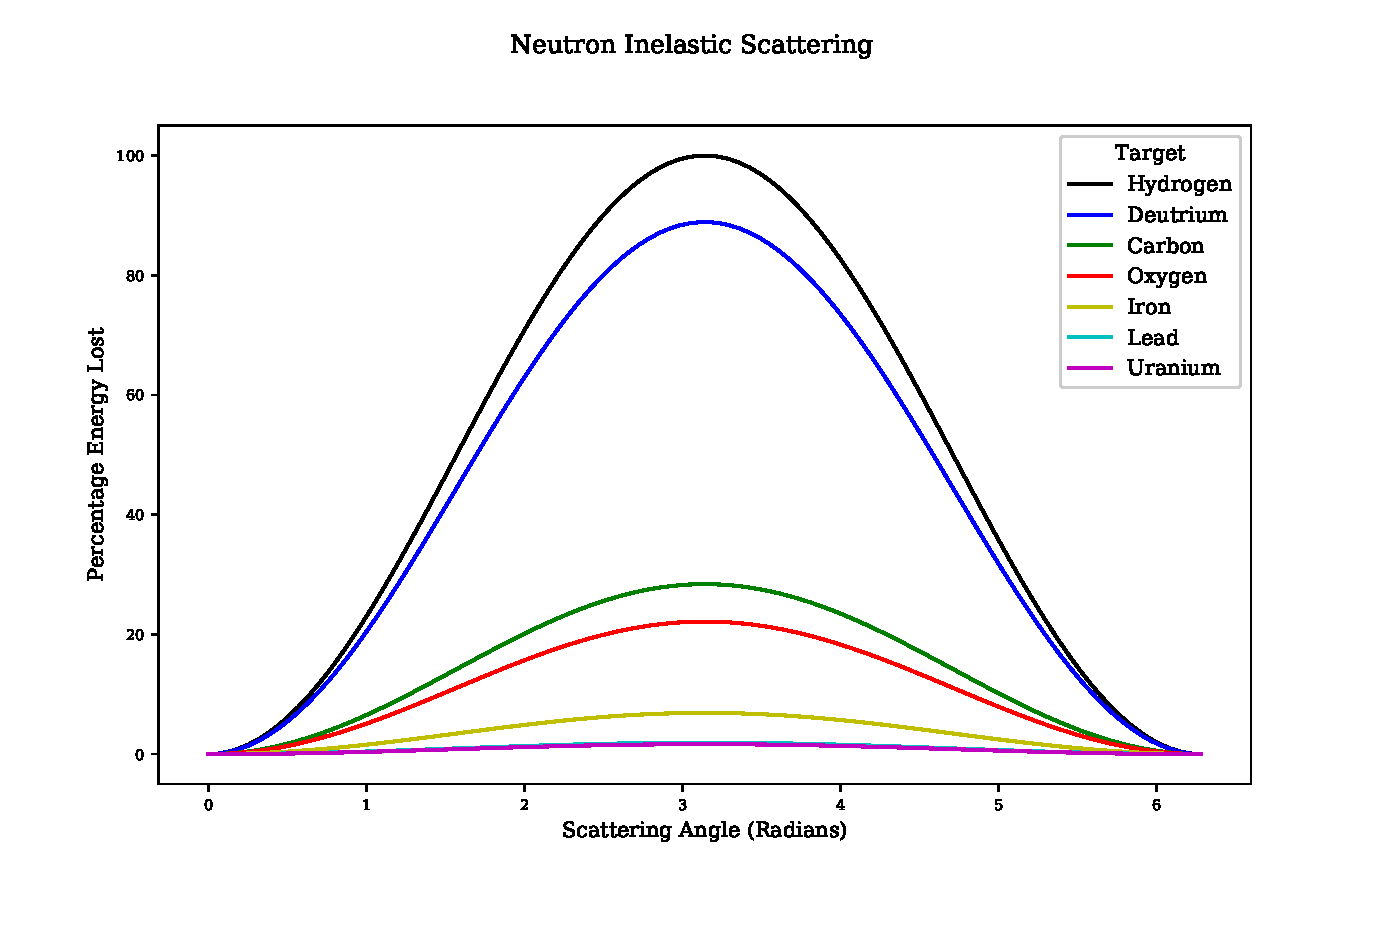
\includegraphics[width=0.7\linewidth]{chapters/introduction/plots/neutron_scattering/neutron_scattering.eps}
    \caption{Inelastic scattering - scattering angle vs energy loss for a range of target atoms - generated with a python script using the equations contained in Duderstadt and Hamilton: Nuclear Reactor Analysis\cite{duderstadthamilton}}
    \label{fig:inelasticscattering}
  \end{center}
\end{figure}

There are several disadvantages to using lead as a coolant.  The melting point of lead is $600K$, so the reactor would need to be heated first for the coolant to become a liquid.  This also restricts the lowest temperature and thus the maximum efficiency possible that may be extracted from the system without the coolant forming a solid.  The density of lead also poses a problem for the structure needed to support the reactor.

\acrfull{elsy} is a 600MWe Lead-Bismuth \gls{eutectic} cooled fast neutron reactor.  It has a lower melting point than lead, but there are concerns for the transmutation of Bismuth to Polonium.  The 9,000 tonne molten lead coolant and the high flux of fast neutrons\cite{lanltour} will be challenging conditions to overcome.



\FloatBarrier
\subsubsection[Very-High-Temperature Reactors]{\acrlong{vhtr}}

Traditional nuclear power plants, as well as coal and the secondary cycle of \acrshort{ccgt} plants, boil water to drive turbines.  \acrfull{vhtr} designs use thermal neutrons and a fissile fuels.  Designs plan to have outlet temperatures of up to $1,270K$\cite{genivgifvhtr}.  With a helium coolant, there are several options.

\begin{itemize}
\item directly drive turbines
\item heat water to create steam and drive turbines
\item use the high temperature to help create hydrogen, and combine with steam driven turbine
\end{itemize}

Hydrogen may be extracted from high temperature water either by a thermo-chemical, high temperature electrolysis or a hybrid process\cite{hydrogenhtr}.  Each process benefits from the very high temperatures provided by the predicted outlet temperatures (fig \ref{fig:energyhydrogenproduction}).

\begin{figure}[!h]
  \begin{center}
    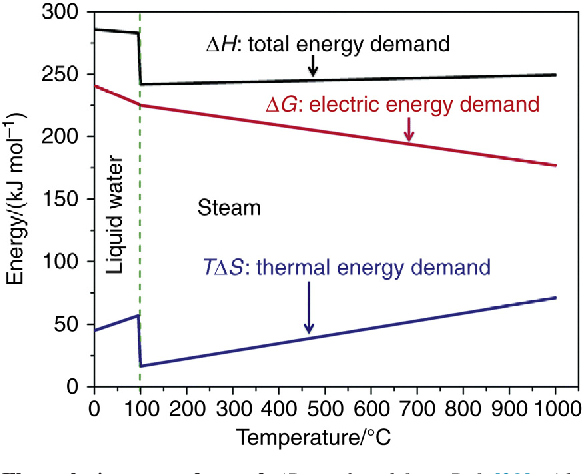
\includegraphics[width=7.0cm]{chapters/introduction/images/hydrogen-from-water.png}
    \caption{Energy demand to produce hydrogen by electrolysis as temperature changes\cite{hydrogenelectrolysis}}
    \label{fig:energyhydrogenproduction}
  \end{center}
\end{figure}

The \acrfull{pbr} is a type of \acrshort{vhtr} where spherical fuel pellets are held in a hopper shaped reactor.  Temperatures within the core may reach $1,770K$, and this will pose a challenge for materials scientists.

\subsubsection[Gas-Cooled Fast Reactors]{\acrlong{gfr}}

The \acrfull{gfr} design is similar to the \acrshort{vhtr}, but rather than use thermal neutrons, it will use fast neutrons.  The design will use a ceramic core and have outlet temperatures up to $1120K$.  This will give similar options to the \acrshort{vhtr} where high temperatures would be used to assist in the production of hydrogen, or it would be used to power a turbine with a secondary steam powered circuit similar to that of a \acrshort{ccgt}.

There are challenges ahead, including the development and testing of advanced materials that can withstand these temperatures while under high energy neutron flux.  However, unlike \acrshort{lfr}s, \acrshort{sfr}s and \acrshort{scwr}s, the coolant is chemically inert and isn't transmuted by neutrons removing the risk of the coolant becoming radioactive.


\FloatBarrier
\subsubsection[Sodium-Cooled Fast Reactors]{\acrlong{sfr}}

Memories of small amounts of sodium, kept under oil in school chemistry labs, being carefully cut and prepared ahead of a violent reaction with water, probably come to mind at the first mention of an \acrfull{sfr}.  It may not be the first choice of an element to use as a coolant, but it does have advantages.  In fact Admiral Rickover once remarked \enquote{if the oceans were filled with liquid sodium, then some crazy scientist would want to build a water-cooled reactor} when the idea of a sodium cooled reactor in a submarine was proposed\cite{atomicaccidents}.

Sodium has a low melting point, of just under $370K$, and a boiling point of $1,150K$.  With an operating temperature of up to $820K$, the reactor would be able to run at atmospheric pressure and without the issues associated with the coolant boiling.  The density of Na is $0.971 gcm^{-3}$ and comparing this to the \acrshort{lfr} the coolant would be 12 times less dense and this would have advantages when designing the structure.

There have been several \acrshort{sfr}s built and operated using this technology, such as the Russian BN-600 reactor.  This particular reactor has a sodium primary loop which heats a secondary sodium loop which in turn heats a third loop for water and steam.




\subsubsection[Super Critical Water Reactors]{\acrlong{scwr}}

At 647K and a pressure of 22.1MPa (approximately 218 atmospheres), water becomes \gls{supercritical} (fig. \ref{fig:waterphasespressuretemp}) and at this point it is neither a liquid or a gas\cite{advancedbiomass}.  The current generation \acrshort{pwr} and \acrshort{bwr} operate at approximately $501-598K$ at 15.2MPa\cite{ocw01} and $551-560K$ at 7.1MPa\cite{ocw02} respectively.

\begin{figure}[!h]
  \begin{center}
    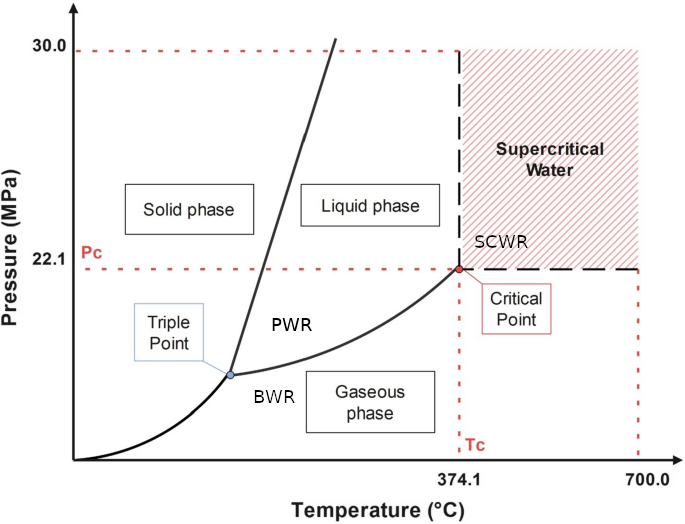
\includegraphics[width=7.0cm]{chapters/introduction/images/supercritical.png}
    \caption{Phases of water:  pressure vs temperature \cite{supercriticalwater}}
    \label{fig:waterphasespressuretemp}
  \end{center}
\end{figure}

Supercritical water exists above $647K$ and 22.1MPa, and in this state water has a higher thermodynamic efficiency.  The design of the nuclear power plant is also simplified as there is no phase change of the water, so a condenser is not needed.  The \acrfull{scwr} is the only \acrshort{gen4} reactor design that uses water as the coolant\cite{gen4}.  The economic benefits have already been seen in SCW fossil fuel power stations, and it is incorporated in \acrshort{gen4} water cooled fast and thermal reactors.  

There are side effects to using supercritical water.  It is an oxidant and is now being considered to \enquote{burn} organic waste in future waste processing plants.  The combination of supercritical water chemistry and irradiation damage must be considered, as well as higher temperature and pressure, when considering the materials used by a \acrshort{scwr}.




\FloatBarrier
\subsubsection[Molten Salt Reactors]{\acrlong{msr}}

\acrshort{msr}s have been operated for over 50 years.  Chemically, salts are very stable, and this has obvious safety benefits over reactors like the \acrshort{sfr}.  The coolants are fluoride salts that have high boiling points which gives the added safety protection of being able to operate at atmospheric pressure, unlike a \acrshort{pwr} where a pressure vessel is needed.

The fuel is dissolved into the molten salt.  There are no solid fuel rods to place into the core, remove or reprocess.  The molten salt is processed on the site to remove poisons, waste and add new fuel.  

\acrshort{msr}s may use either thermal or fast neutrons and a range of fuels including \Gls{Th}.  This is particularly interesting as Th is three times as abundant as U and would increase the fuel available to us for the clean production of electricity by nuclear power.

A safety feature that takes advantage of the fuel being dissolved in the molten salt are large drain tanks under the reactor.  A plug is designed to melt if it reaches a certain temperature and this would quickly drain the molten salt from the reactor into large and cold drainage tanks.  The reactivity would drop and the fuel would cool reverting it to a solid salt. 

Salts considered in various designs are chlorides, nitrates and fluorides.  Corrosion of the reactor due to the molten salts is a concern.  Elements that provide protection to corrosion, such as Cr, are prone to dissolution into the molten salt\cite{msrcorrosion}.  Where the fuel is suspended in the molten salt as \acrfull{triso} fuel particles, formation of chromium-carbide precipitates may be an issue.


\FloatBarrier
\subsubsection{Experimental Fusion Reactors}

Nuclear Fusion is a very attractive technology and could be the answer to all of our energy problems.  Much work is being invested in developing this technology and the \acrfull{iter} has been designed to output more energy than is required to start the fusion reaction.  The process of fusion combines two isotopes of hydrogen and creating helium, fast neutrons (eq. \ref{eq:fusionreaction}) and an excess of energy.  As neutrons have no charge, they can penetrate shielding causing damage as they lose energy through nuclear interactions.   Any atoms they interact with have a chance to capture the neutron and become unstable.

\begin{equation}
_{1}D^{2} + _{1}T^{3} \to _{2}He^{4} (3.5MeV) + _{0}n^{2} (14.1MeV)
\label{eq:fusionreaction}
\end{equation}

The fast neutron spectrum for fission reactors ranges from a few eV to a few MeV, whereas the neutrons in a fusion reaction have 2-3 times more energy than the most energetic neutrons from fast fission.  Engineers must develop materials to construct components that will be resilient to this damage, while having a low reaction cross section and being able to withstand other extreme conditions within the reactor.  

Unfortunately, nuclear fusion as a commercial method of creating energy, is often said to be 30 years away, and this has been the case for some time now.  It is a lot to ask, recreating a process that occurs within a star, in a safe and steady manner.  Once this problem is solved, it could mark a turning point for human civilization.




%%%%%%%%%%%%%%%%%%%%%%%%%%%%%%%%%%%%%%%%%%%%%%%%%%%%%%%%%%%%%%%%%%%%%%%%%%%%%%%%%%%%%%%%%%%%%%%%%%%%%%%%%%
%%
%%  REACTION AND NEUTRON SPECTRA
%%  
%%%%%%%%%%%%%%%%%%%%%%%%%%%%%%%%%%%%%%%%%%%%%%%%%%%%%%%%%%%%%%%%%%%%%%%%%%%%%%%%%%%%%%%%%%%%%%%%%%%%%%%%%%


\FloatBarrier
\section{Damage to Nuclear Core Components by Neutrons}

Radiation damage in a reactor is caused by several projectiles.  Fission fragments are heavy, contain charged particles and lose energy close to their source.  Gamma rays excite electrons, promoting them to higher energy levels, or ionise the atoms where there is enough energy to eject electrons completely from atoms.  They do not have the momentum to knock atoms out of place.  Fast neutrons, however, may impart a great deal of momentum to a target atom and, as they are neutral, travel much further into a material than fission fragments.  With enough energy, neutrons cause large damage cascades within the material.

One fuel source for many of the \acrshort{gen3+} and \acrshort{gen4} reactors is ${}^{235}_{92}U$, whether as enriched U or otherwise.  The neutron(s) released by the fission of ${}^{235}_{92}U$ atoms have a spectra of energy (fig. \ref{fig:neutronfissionspectra}) which may roughly be split into four categories: cold (below 0.025eV), thermal (0.025eV), slow and intermediate (above 0.025eV and below 1MeV) and fast (1MeV and above).

\begin{figure}[!h]
  \begin{center}
    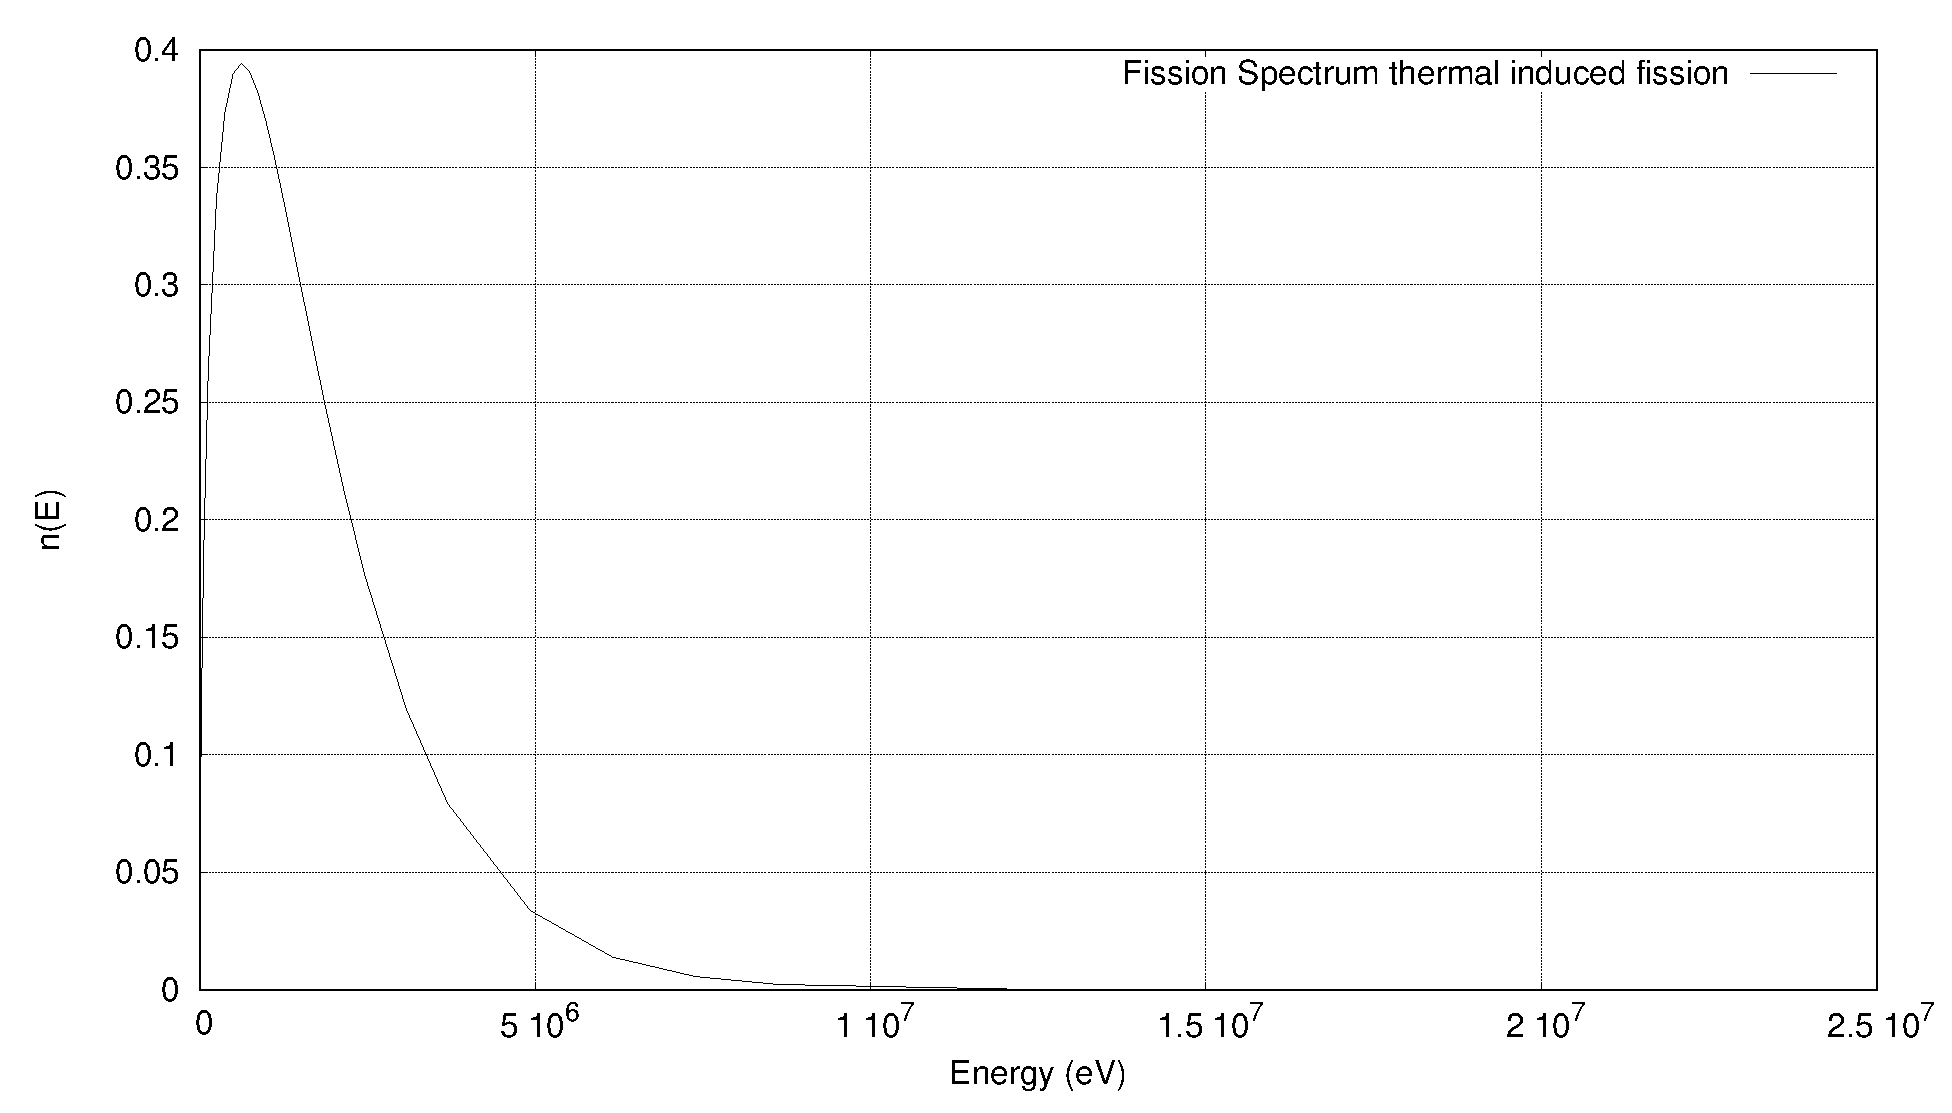
\includegraphics[width=10.0cm]{chapters/introduction/plots/fission_spectra/fission_spectra.eps}
    \captionsetup{font={it}}
    \caption{Neutron energy spectrum from fission generated from the JEFF 3.1.1 data file\cite{jeff311}}
    \label{fig:neutronfissionspectra}
  \end{center}
\end{figure}

Thermal and slow/intermediate neutrons cause damage in their own particular way, as they are captured by and transmute the atoms within the target material.  Fast neutrons have enough energy to create a great deal of damage, whereby they transfer kinetic energy to an atom in the material that becomes the \acrfull{pka} in a cascade of atoms through the material.  Neutrons can travel deep into a material, creating many damage cascades throughout until they lose enough energy or pass through completely.

\begin{figure}[!h]
  \begin{center}
    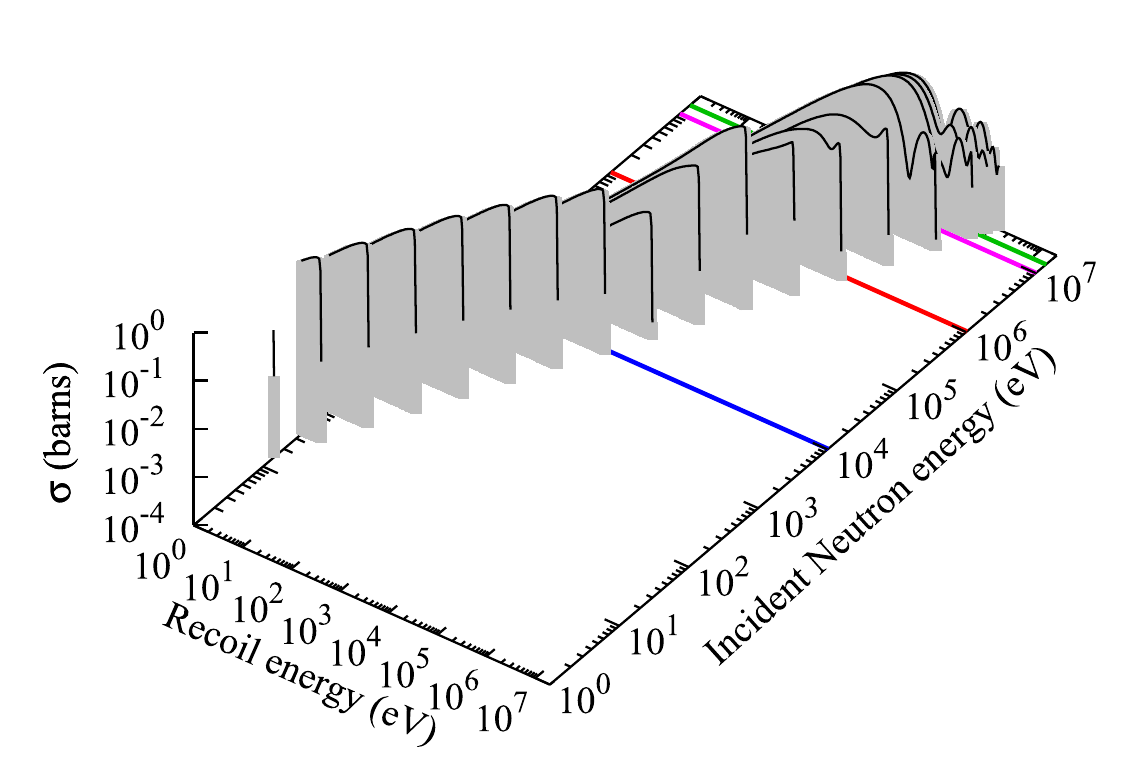
\includegraphics[width=10.0cm]{chapters/introduction/plots/damage/pkaenergy.png}
    \captionsetup{font={it}}
    \caption{\acrshort{pka} energy as a funtion of neutron energy in Fe\cite{pkaenergyspectra}}
    \label{fig:neutronironrecoil}
  \end{center}
\end{figure}

The intensity of neutron energies from the fission of ${}^{235}_{92}U$ peaks around 1MeV (fig. \ref{fig:neutronfissionspectra}).  The energy transferred to \acrshort{pka}s will vary depending on the mass of the target nucleus and scattering angle but, in Fe at least, 1MeV neutrons will create the majority of its Fe \acrshort{pka}s with energies ranging from 1keV to 100keV (fig. \ref{fig:neutronironrecoil}).




%%%%%%%%%%%%%%%%%%%%%%%%%%%%%%%%%%%%%%%%%%%%%%%%%%%%%%%%%%%%%%%%%%%%%%%%%%%%%%%%%%%%%%%%%%%%%%%%%%%%%%%%%%
%%
%%  Ion Irradiation
%%  
%%%%%%%%%%%%%%%%%%%%%%%%%%%%%%%%%%%%%%%%%%%%%%%%%%%%%%%%%%%%%%%%%%%%%%%%%%%%%%%%%%%%%%%%%%%%%%%%%%%%%%%%%%




\FloatBarrier
\section{Radiation Damage: Replacing Neutrons with Protons}

It is difficult to generate large fluxes of neutrons.  Neutrons have no net charge, so they cannot be controlled in a similar way.  Nuclear reactors are the most common way to create large fluxes of neutrons.

This an expensive method, and one that may be inconvenient as the sample being tested would need to be placed inside a reactor.  Rather than do this, ions may be used to replicate the damage cause by neutrons, but in a more controlled and accessible way.

Experimental reactors are not able to damage a material significantly faster than operational reactors, so a major reason for approximating with ion irradiation is the higher damage rate, with the hope of discovering potential problems before they manifest in current reactor designs\cite{wasionchallenges}. 

The damage caused by neutrons, light ions and heavy ions differ due to their interactions with matter.  Ions lose energy gradually but within a very short distance, whereas neutrons lose larger amount of energy less frequently, but over much greater distances.  The \acrshort{pka} energies as a result are higher for neutrons than ions, however comparisons of low damage dose neutron and light ion irradiation show cluster size distribution to be independent of \acrshort{pka} energies\cite{wasionchallenges}\cite{primarydamageiron}.

A major side effect from the process of nuclear fission is the creation of both radioactive fission fragments and radioactive isotopes within the components and structural material of the reactor.  Low energy protons are not captured as low energy neutrons would be, due to the opposing electromagnetic force between the proton and nucleus of the target atom.  Once the proton energies exceed a few MeV, they have sufficient energy to transmute target nuclei.

The benefits of ion irradiation as discussed, and positive studies into the independence of damage due to \acrshort{pka}s in the energy range 6.6keV to 176keV\cite{primarydamageiron}, support its use in emulating neutron damage.

Induced radioactivity is still a problem.  By virtue of detailed reaction cross section data files and decay data, the amount of radioactivity induced by both protons and neutrons may be calculated.  This will assist in the selection of proton beam parameters to replicate irradiation damage, to the required \acrshort{dpa}, whilst keeping the radioactivity at a safe level.


%%%%%%%%%%%%%%%%%%%%%%%%%%%%%%%%%%%%%%%%%%%%%%%%%%%%%%%%%%%%%%%%%%%%%%%%%%%%%%%%%%%%%%%%%%%%%%%%%%%%%%%%%%
%%
%%  Molecular Dynamics
%%  
%%%%%%%%%%%%%%%%%%%%%%%%%%%%%%%%%%%%%%%%%%%%%%%%%%%%%%%%%%%%%%%%%%%%%%%%%%%%%%%%%%%%%%%%%%%%%%%%%%%%%%%%%%


\FloatBarrier
\section{Simulated Material Damage}

Irradiating and testing materials with both neutrons and protons has a number of drawbacks, including expensive facilities and the creation of radioactive waste.  Simulations may be used to help understand the processes on a mesoscopic scale and make predictions on how the materials in question may behave inside a reactor under certain conditions.

Part of this work focuses on the damage of stainless steel by neutrons.  The damage process occurs on time scales and sizes too small to capture experimentally and play back to study.  The theories may not be sufficiently well understood, or are often unsolvable with current techniques.  Modelling helps bridge the gap between theory and experiment. 

\subsection{Molecular Dynamics}
 
Molecular dynamics models have been used to simulate radiation damage.  Damage cascades caused by \acrfull{pka}s with energies of 10, 20 and 50KeV have been modelled in \acrshort{bcc} \Gls{W}\cite{damagebcctungsten}, whilst cascades caused by \acrshort{pka}s of 5, 10 and 20KeV have been simulated in \acrshort{bcc} Fe\cite{damagebcciron}.

Neutrons have a long mean path before interacting with a target when compared to ions.  It would be impossible with current and foreseable technology to simulate a neutron travelling through a material because the volume of the material, and the number of atoms and interactions between atoms, would be so large.  Rather than attempt this, it is more productive to focus on individual damage cascades caused by \acrshort{pka}s in order to conserve computing resources.

\begin{figure}[!h]
\begin{subfigure}{.5\textwidth}
  \centering
  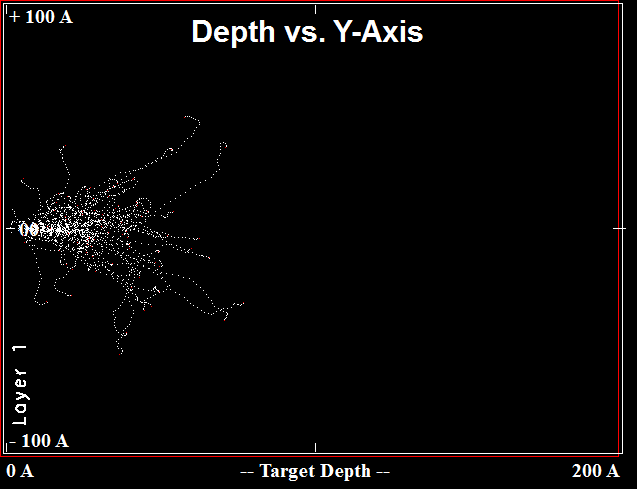
\includegraphics[width=.7\linewidth]{chapters/introduction/images/5KeV.png}
  \caption{5KeV Fe PKA damage cascade in Fe} 
\label{fig:damagecascade5kev}
\end{subfigure}
\begin{subfigure}{.5\textwidth}
  \centering
  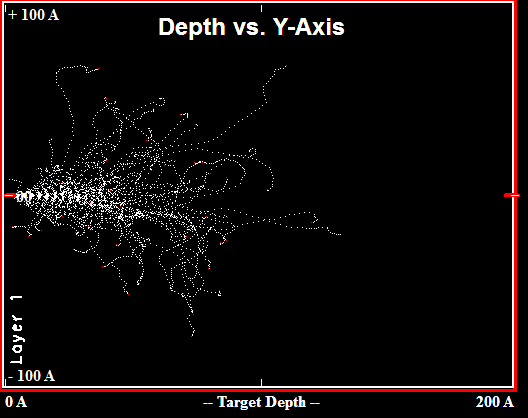
\includegraphics[width=.7\linewidth]{chapters/introduction/images/10KeV.png}
  \caption{10KeV Fe PKA damage cascade in Fe} 
  \label{fig:damagecascade10kev}
\end{subfigure}
\begin{subfigure}{.5\textwidth}
  \centering
  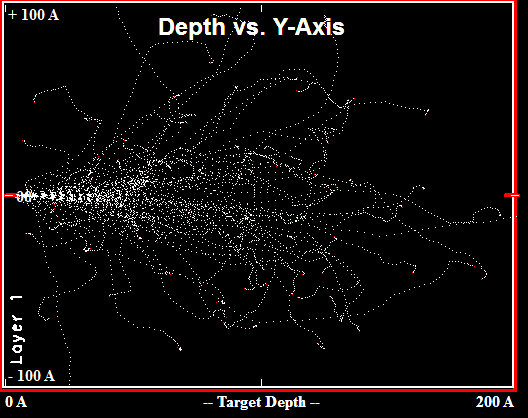
\includegraphics[width=.7\linewidth]{chapters/introduction/images/20KeV.png}
  \caption{20KeV Fe PKA damage cascade in Fe} 
  \label{fig:damagecascade5kev}
\end{subfigure}
\begin{subfigure}{.5\textwidth}
  \centering
  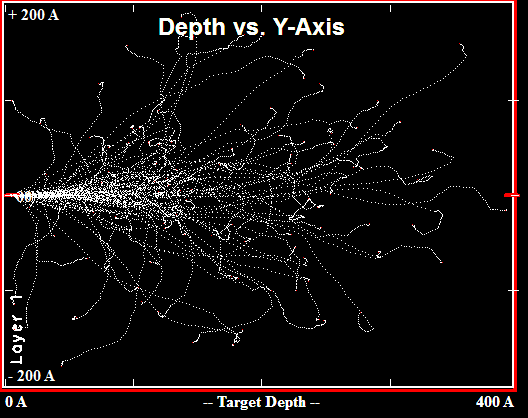
\includegraphics[width=.7\linewidth]{chapters/introduction/images/50KeV.png}  
  \caption{20KeV Fe PKA damage cascade in Fe} 
\label{fig:damagecascade10kev}
\end{subfigure}
\caption{Damage cascades in Fe for a range of energies generated in \acrshort{srim}\cite{srim}}
\label{fig:damagecascades}
\end{figure}

Molecular Dynamics simulations require interatomic potentials to govern how the atoms in the simulation interact with one another.  Typical simulation sizes range from thousands of atoms to millions of atoms.

Fe has a density of approximately $8.5 \times 10^{-2}$ atoms per cubic angstrom, and this leads to simulation sizes between almost one million atoms and fifty million atoms for cascades with \acrshort{pka}s ranging from 5KeV to 50KeV (fig \ref{fig:damagecascades}, table \ref{table:fesimulationsize}).

\begin{table}[h]
\begin{center}
\renewcommand{\arraystretch}{1.2}
\begin{tabular}{c c c}
\hline\hline
PKA Energy (KeV) & Volume $(Ang^3)$ & Atoms \\
\hline\hline
5 & $1.0\times 10^6$ & $9.0\times 10^5$ \\
10 & $6.0\times 10^6$ & $5.4\times 10^6$ \\
20 & $8.0\times 10^6$ & $6.9\times 10^6$ \\
50 & $6.4\times 10^7$ & $5.5\times 10^7$ \\
\hline\hline
\end{tabular}
\end{center}
\caption{Simulation sizes by PKA energy approximated using \acrshort{srim}\cite{srim}}
\label{table:fesimulationsize}
\end{table}

The interatomic potentials used to simulate a damage cascade must be able to model the very close separations during the collisions event.  For very close separations, an exponential potential such as the \acrfull{zbl} potential may be used, and for other separations a standard potential such as the \acrfull{eam} may be used, in particular for metals.

There have been attempts to create potentials based on Physics, but the nuances are still poorly understood and there aren't any models that can be applied accurately to any material type under any set of circumstances.  A number of recent interatomic potentials, including a selection of transition metals, have been fit to match the experimental data rather than the underlying physics.


\subsection{Density Functional Theory}

In Quantum Mechanics, the Schr\"{o}dinger equation and the wavefunction of a system describes all that can be known about that quantum system.  Unfortunately, it is very difficult to compute when there are just several electrons in the system.  Many atoms in a system makes this an impossible task with current technology.

\acrfull{dft} replaces the many electron wavefunction with many single electron wavefunctions.  Rather than use the positions of all the electrons, which would result in $3^n$ parameters, the charge density is used.  It is important to note that \acrshort{dft} is an exact method for ground state calculations, although in practice approximations do need to be made in order to solve problems.  This is discussed in detail in section \ref{section:dftbackground}.


\subsection{Interatomic Potentials for Molecular Dynamics}

Interatomic potentials help to describe the interaction between atoms.  Originally they were used for pairs of atoms and a collection of atoms on a pair by pair basis, but in the 1980s the complexity of potentials increased as they started to include the effects of the background electron density that the atoms are embedded in.  This lead to the \acrfull{fs} and \acrfull{eam} type potentials.

Whilst \acrshort{dft} is a purer form of computational materials science, more closely linked to physics, it is computationally intensive and suitable for small systems of hundreds to thousands of atoms.  By using interatomic potentials to recreate the forces and energies that would be computed by \acrshort{dft}, the systems may be increased in size to thousands to millions of atoms, and these calculations may be run over a time frame with hundreds or thousands of time steps.

There are a wide range of potentials, and these are typically selected based on the type of material and the required accuracy.  Simple pair potentials may still be used, but angularly dependent potentials have been developed for materials with covalent bonds, and metals use \acrshort{fs} and \acrshort{eam} potentials.  The potentials are made up of a set of functions, and these functions change from derivation to derivation.  




%%%%%%%%%%%%%%%%%%%%%%%%%%%%%%%%%%%%%%%%%%%%%%%%%%%%%%%%%%%%%%%%%%%%%%%%%%%%%%%%%%%%%%%%%%%%%%%%%%%%%%%%%%
%%
%%  Scope and Objectives
%%  
%%%%%%%%%%%%%%%%%%%%%%%%%%%%%%%%%%%%%%%%%%%%%%%%%%%%%%%%%%%%%%%%%%%%%%%%%%%%%%%%%%%%%%%%%%%%%%%%%%%%%%%%%%

%%\section{Scope and Objectives}



